\chapter{Teoretický základ}
\label{2-teorie} Tato kapitola se zabývá základy ionizujícího záření,
jeho zdroji a biologickými účinky. Dále je popsána činnost mobilních
skupin provádějících pozemní monitorování radiace. Poslední část
kapitoly stručně pojednává o~přínosu této bakalářské práce a~tvoří
přechod mezi teoretickou a~praktickou částí.

\section{Ionizující záření}
	
Záření (radiace) je proces, při kterém energie prochází
prostorem. Typickými pří\-klady záření, se kterými se setkáváme na denní
bázi, je sluneční svit, rádiový, televizní nebo i wifi signál.

Ionizující záření je záření s~takovým množstvím energie, že může
vyrážet elektrony z~atomového obalu a tím látku ionizovat. Tento jev
se využívá například v~radiologii, lékařském oboru, který ionizující
záření používá za účelem diagnóz, terapií a rozvoje vědy. \citep{who}

\subsection{Druhy ionizujícího záření} Ionizující záření se dělí na
dva druhy: \cite{ionZarUllman} \cite{CEZ}

\begin{itemize}
	\item \textbf{Přímo ionizující}
	
		Kvanta přímo ionizujícího záření nesou elektrický
náboj a přímo vyrážejí elektrony z~atomů. Součástí této kategorie je
např. záření $\alpha$ (prudce letící kladná jádra izotopu helia
$_{2}He^{4}$), $\beta^{-}$ (proud elektronů vznikající při přeměně
neutronu na proton), $\beta^{+}$ (proud kladných pozitronů, antičástic
k~elektronům) atd.
		 
	\item \textbf{Nepřímo ionizující}
	
		Nepřímo ionizující záření předává svou kinetickou
energii nabitým látkovým částicím, které pak látku ionizují. Kvanta
tohoto záření tedy nejsou elektricky nabita. Do této kategorie se řadí
především rentgenové a $\gamma$ záření (elektromagnetická záření
s~velmi nízkou vlnovou délkou).
\end{itemize}

\subsection{Fyzikální jednotky} V~jaderné fyzice se jako základní
jednotka používá becquerel [Bq] patřící mezi odvozené jednotky
soustavy SI. Vyjadřuje střední počet radioaktivních přeměn za
sekundu. Tato jednotka ovšem neříká nic o~druhu záření, jeho
biologickém účinku, energii atd. Pro popis ionizujícího záření jsou
zavedeny veličiny, které slouží jako charakteristiky jeho účinků na
různé látky. \cite{atomInfo}

\begin{itemize}
	\item \textbf{Dávka, dávkový příkon}
	
		 Nejdůležitější z~těchto veličin je tzv. dávka, která
má za jednotku gray [Gy] patřící mezi jednotky SI. Fyzikální
rozměr jednotky gray je joule na kilogram [J/kg]. Častá veličina je
 tzv. dávkový příkon, tedy přírůstek dávky v~čase [Gy/s].
		
	\item \textbf{Ekvivalentní dávka, ekvivalentní dávkový příkon}

	 	V~předchozím bodě zmíněné veličiny nezohledňují
všechny účinky působení záření na živou hmotu. Proto byly zavedeny
radiobiologické veličiny. Patří sem ekvivalentní dávka, která je
vypočtena z~dávky přenásobené tzv. jakostním činitelem Q závisejícím
na typu a energii záření. Hodnota Q je doporučovaná mezinárodní komisí
radiologické ochrany\footnote{V dokumentu ICRP Publication 103
dostupném na
\url{http://www.sujb.cz/fileadmin/sujb/docs/radiacni-ochrana/ICRP103\_dokument.pdf}}. Například
u~gama záření je Q = 1. Ekvivalentní dávka má za jednotku sievert
[Sv], ekvivalentní dávkový příkon pak sievert za jednotku času [Sv/s].
	 	
	\item \textbf{Shrnutí jednotek}
	
		\begin{table}[h!]  \centering
			\caption{Fyzikální jednotky ionizujícího
záření}
			\label{tab:tabulkaJednotek}
			\begin{tabular}{|c|c|c|} \hline \textbf{Název}
& \textbf{Jednotka} & \textbf{Značení} \\ \hline Dávka & gray &
{[}Gy{]} \\ \hline Dávkový příkon & gray za sekundu & {[}Gy/s{]} \\
\hline Ekvivalentní dávka & sievert & {[}Sv{]} \\ \hline Ekvivalentní
dávkový příkon & sievert za sekundu & {[}Sv/s{]} \\ \hline
			\end{tabular}
		\end{table}
\end{itemize}

\subsection{Zdroje ionizujícího záření} Zdroje ionizujícího záření
mohou být přírodní a umělé. Největší ozáření obyvatelstva způsobují
zdroje přírodní, přestože pozornost je věnována především zdrojům
umělým. \cite{radiobiologie}

\begin{itemize}
	\item \textbf{Přírodní zdroje záření}
	
			Tyto zdroje tvoří tzv. přírodní
pozadí. Přírodní zdroje jsou dále rozděleny na dvě kategorie, kosmické
záření a přírodní radionuklidy.  Množství kosmického záření se odvíjí
od nadmořské výšky a zeměpisné šířky kvůli působení zemského
magne\-tického pole na dráhu nabitých částic. Například mezi 30$^{o}$ a
60$^{o}$ jižní resp. severní šířky je intenzita záření příbližně
o~10\% vyšší než na rovníku a magnetických pólech.  Zdroje přírodních
radionuklidů jsou především horniny. Intenzita záření se odvíjí od
původů jednotlivých hornin. Pro ilustraci, vyvřelé horniny vykazují
vyšší aktivitu než horniny metamorfované.
	
	\item \textbf{Umělé zdroje záření}
	
			Za umělé zdroje záření jsou považovány takové
zdroje, které způsobují ozáření při činnostech s~nimi, dále takové
zdroje, které souvisí s~lékařskými zákroky. Běžně se vedle lékařského
ozáření další zdroje podílí na ozáření člověka pouze
minimálně. Dalšími zdroji jsou radionuklidy nacházející se v~životním
prostředí pocházející ze spadu po mimořádných jaderných haváriích
(poškození jaderného zařízení) nebo po zkouškách jaderných
zbraní. Radionuklidy, které se dostaly do ovzduší, se dostávají na
povrch ve formě suchého nebo mokrého spadu s~deštěm, kde kontaminují
vodu a potravu.
			
\end{itemize}

Podrobnější popis zdrojů ionizujícího záření by byl nad rámec této
bakalářské práce, proto nebude dále rozebírán.

\subsection{Biologické účinky ionizujícího záření} Pro stanovení
kritérií a principů radiační ochrany obyvatelstva a pracujících, kteří
přicházejí se zdroji ionizujícího záření více do kontaktu, je potřeba
vědět, jak ioni\-zující záření působí na lidský organismus. Z~těchto
kritérií je dále odvozen systém limitování dávek (viz. kapitola
\ref{sub:limity}). \cite{sujbBiologickeUcinky}

Jak již bylo stručně popsáno, ionizující záření (radiace) způsobuje
ionizaci atomů. Ta může dále vést k~chemickým reakcím, fyzikálním
změnám a v~případě živých tkání k~biochemickým změnám. Tyto změny
mohou vést k~poškození organismu nebo~i~k~jeho úmrtí. Účinek radiace
na organismus je rozdělen na 4 následující etapy: \cite{bioZarUllman}
\newpage
\begin{enumerate}
	\item \textbf{Fyzikální stádium}
	
		Fyzikální stádium je primární proces, při kterém
dochází k~ionizaci atomů (což vede k~narušení chemických vazeb mezi
atomy a molekulami). Při dávce 1Gy se v~objemu každé ozářené buňky
o~typické velikosti 10$\mu$m vytváří 10$^5$ ionizací. Tento proces
trvá jen cca 10$^{-16}$ - 10$^{-14}$s.
		
	\item \textbf{Fyzikálně-chemické stádium}
	
	Sekundárním procesem je fyzikálně-chemické stádium, při kterém
dochází k~disociaci molekul (rozklad na kladně a záporně nabité
částice) a vzniku volných radikálů (vysoce reaktivních částic). Tento
proces je podobně jako proces předchozí velmi rychlý. Trvá přibližně
10$^{-14}$ - 10$^{-10}$s.
	
	\item \textbf{Chemické stádium}
	
	Produkty předchozích stádií reagují s~důležitými organickými
molekulami a mění jejich složení a funkci. Například zlomy řetězců
v~molekule DNA jsou řazeny mezi typické poruchy. Trvání tohoto stádia
ovlivňuje transportní doba reaktivních složek z~místa svého vzniku do
místa napadené biomolekuly v~rozmezí od tisícin sekundy do řádově
jednotek sekund.
	
	\item \textbf{Biologické stádium}
	
	Popsané molekulární změny mohou vyústit ve funkční a
morfologické změny v~buňkách, orgánech a poté i celkově
v~organismu. Trvání této fáze se pohybuje od jednotek sekund (buňky)
až po několik let (organismus). Kdy se biologické stádium projeví,
záleží na množství dávky záření. Při nízkých dávkách se může projevit
až za několik desítek let, kdežto naopak při vysokých dávkách již
během desítek minut.
\end{enumerate}

Lidský organismus má omezenou schopnost opravy poškozených molekul
buněk. Pokud však dávka překročí určitou mez, buňky uhynou a vzniká
tzv. nemoc z~ozáření.


Nemoc z~ozáření může být rozdělena na 2 kategorie: \cite{nemoc}

\begin{itemize}
	\item \textbf{Akutní nemoc z~ozáření}
	
		Akutní nemoc z~ozáření je způsobena jednorázovým
ozářením. Prvotními pří\-znaky jsou nevolnost, zvracení a průjmy. Pokud
dávka ozáření překročí hodnotu přibližně 4 Sv, nastupuje tzv. střevní
forma, kterou doprovází krvavé průjmy a mine\-rální rozvrat. Poté
přichází období latence (prodlevy), jehož délka trvání závisí na
množství absorbované dávky. Po uplynutí latentní fáze nastupuje
tzv. dřeňová forma, kdy dojde k~zhroucení krvetvorby a imunitních
mechanismů. Nemoc v~této fázi dále způsobuje sepsi, sterilitu,
u~těhotných žen potrat atp. Pokud dojde k~absorpci dávek záření
vyšších než 10 Sv, dochází k~nevratnému poškození buněk centrálního
nervového systému a později nastává smrt.
		
	\item \textbf{Chronická nemoc z~ozáření}
	
		Tato forma nemoci z~ozáření se rozvíjí při dlouhodobém
působení malých dávek ionizujícího záření. Dále se dělí na 3
fáze. První z~nich je fáze nespecifických obtíží způsobující
nespavost, bolesti hlavy, pokles počtu bílých krvinek, zažívací obtíže
atd. Další z~fází je fáze výrazné symptomatologie, kde se stupňují
bolesti hlavy, dochází k~poruchám motoriky, k~chronickým průjmům,
váhovým úbytkům atd. Dochází k~poškození centrálního nervového
systému, což doprovází zhoršený sluch a zrak. Následuje poslední fáze
nezvratného poškození. Přestávají fungovat rozmnožovací orgány,
dochází k~poškození srdce, ledvin, jater, dále se na kůži a~sliznici
tvoří vředy atd.

\end{itemize}

\section{Radiační ochrana} Cílem radiační ochrany je zajistit ochranu
obyvatelstva před účinky ionizujícího záření a zároveň umožnit
z~těchto účinků vytěžit co největší přínos (v~radiologii, v~jaderné
energetice atp.). Důležitou součástí radiační ochrany je monitorování
radiační situace. Nasbíraná data slouží pro posuzování stavu ozáření,
pro další potřeby sledování a pro rozhodování o~opatřeních v~případě
radiačních havárií. \cite{suroRadOch} \cite{sujbRadSit}

\subsection{Limity expozice ionizujícímu záření v~České republice}
\label{sub:limity} Stupeň povoleného ozáření obyvatelstva se řídí
omezeními, která jsou určována le\-gislativou ve vyhláškách úřadů
zabývajících se touto problematikou (\zk{SÚRO}, \zk{SÚJB}). Konkrétně
pro Českou republiku je to vyhláška 307/2002 Sb. Na základě doporučení
pracovníků SÚRO jsou hodnoty dávky resp. dávkového příkonu udávané
v~jednotkách microsievert [$\mu$Sv] resp. microsievert za hodinu
[$\mu$Sv/h]. Limity expozice ionizujícímu záření v~ČR jsou patrné
z~obrázku \ref{fig:davkyCR}. \cite{suroPriRadOch}

\begin{figure}[H] \centering
    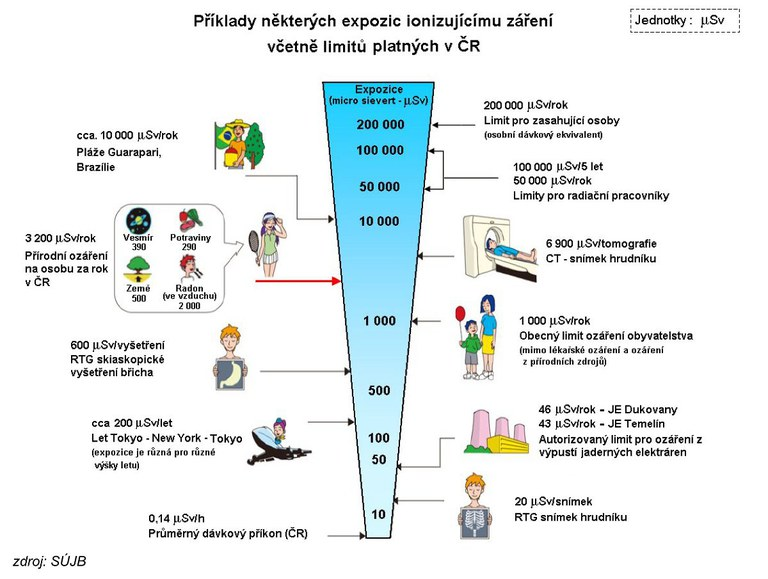
\includegraphics[scale=0.6]{./pictures/davkyCR.jpeg}
      	\caption[Příklady expozice a limity]{Příklady expozice a
limity (zdroj: \cite{suroOcek})}
    	\label{fig:davkyCR}
\end{figure}

\subsection{Pozemní monitorování radiační situace} Pomocí
tzv. Radiační monitorovací sítě (\zk{RMS}) je zjišťována radiační
situace na území České republiky. Na činnosti \zk{RMS} se podílejí
resorty různých ministerstev (financí, obrany, vnitra atd.), dále
držitelé povolení k~provozu jaderných zařízení a~hlavně Státní ústav
radiační ochrany (\zk{SÚRO}). Řízením je pověřen Státní ústav pro
jadernou bezpečnost (\zk{SÚJB}). \cite{suroRMS}

Součástí \zk{RMS} jsou i mobilní skupiny (\zk{MS}), jejichž úkolem je
dodat krizovému štábu při radiačních haváriích (radiační nehoda
vyžadující opatření na ochranu obyvatelstva a životního prostředí)
dostatek dat pro posouzení radiační situace a návrh nutných
opatření. \zk{MS} při jízdě autem kontinuálně monitorují ekvivalentní
dávky resp. ekvivalentní dávkové příkony (pro zjednodušení dále
v~textu jako dávky resp. dávkové příkony), odebírají vzorky složek
životního prostředí atd.  \cite{metodika} \cite{pecha2011monitorovani}

\begin{figure}[H] \centering
    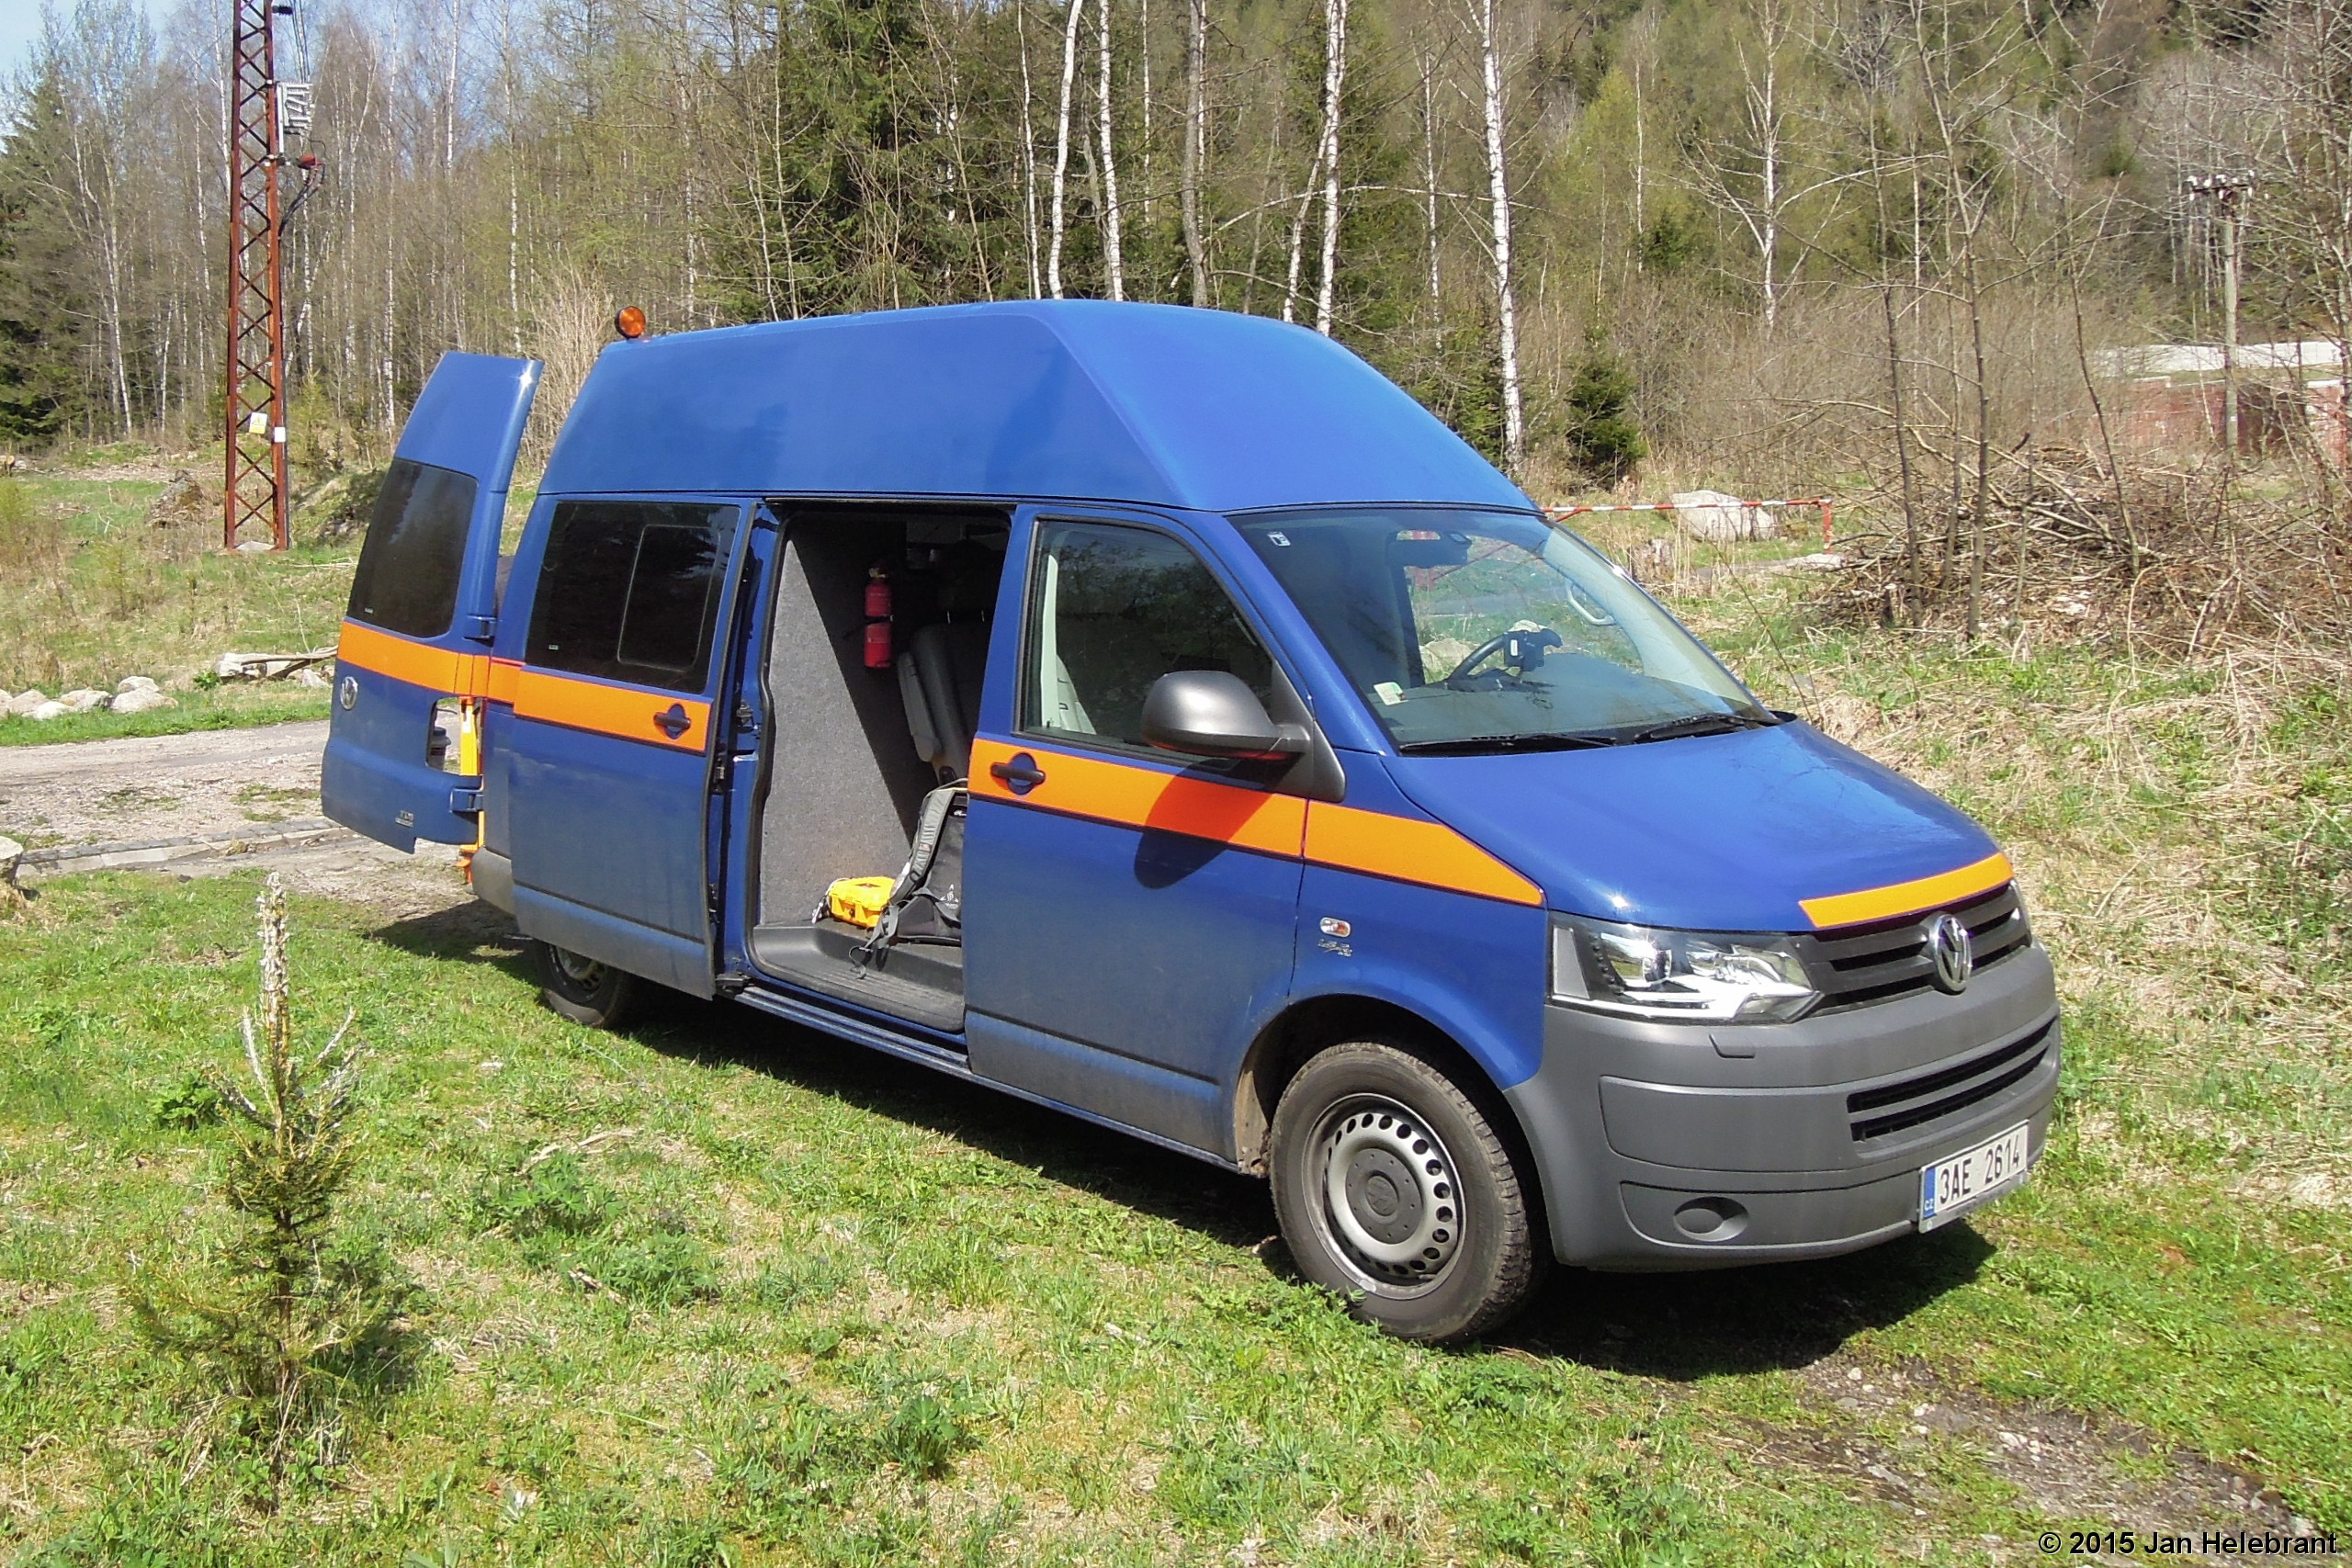
\includegraphics[scale=0.6]{./pictures/vuzSURO.jpg}
      	\caption[Vůz \zk{MS} \zk{SÚRO} Praha]{Vůz \zk{MS} \zk{SÚRO}
Praha (zdroj: SÚRO, v.v.i.)}
    	\label{fig:vuzSURO}
\end{figure}

Před vlastním únikem škodlivých látek do ovzduší při radiačních
haváriích jsou k~dispozici modelové prognózy vznikající radiační
události získané na základě napočítaných havarijních sekvencí,
reálných údajů a meteorologické situace. Vedle těchto modelů jsou již
v~době úniku měřeny hodnoty dávkových příkonů ze sítě dozimetrů
(zařízení k~měření dávek ionizujícího záření) rozmístěných
po areálu jaderné elektrárny. Všechny tyto informace napomáhají
krizovému štábu identifikovat směr úniku a vytipovat oblasti
monitoringu pro \zk{MS}.

\subsubsection{Fáze radiační havárie}

Radiační havárie v~jaderné elektrárně (a její řešení) je rozdělena na
3 hlavní fáze:

\begin{itemize}
	\item \textbf{Časná fáze}
	
		Časná fáze zahrnuje dobu přibližně 1-2 dnů po ukončení
úniku látek z~havarované jaderné elektrárny. Během této fáze je nutné
co nejdříve zmapovat dávkové příkony na daném území. Pro lepší
komunikaci mezi krizovým štábem a \zk{MS} jsou předpřipravené trasy,
které jsou dále upravovány podle naměřených hodnot. Blízké okolí
jaderných elektráren (20km JE Dukovany, 13km JE Temelín) je rozděleno
na 16 sektorů. V~každém sektoru je právě pro prvotní fázi monitorování
připravena 1 trasa monitorování zasahující i do sektorů
vedlejších. Vytipována je ještě 17. pojezdová trasa, která je vedena
po blízkém okolí jaderné elektrárny. Cílem časné fáze je pomocí
měřených hodnot v~daném místě a čase upřesnit modelovou prognózu a
získat tak podklady pro rozhodování o~evakuaci obyvatelstva.

	\item \textbf{Střední a pozdní fáze}
		
		Střední a pozdní fáze může mít v~závislosti na
závažnosti havárie trvání několik týdnů až roků. Tato fáze má za cíl
získat podklady k~rozhodnutí o~dalších ochranných opatřeních, ukončení
evakuace, regulaci potravních řetězců, přesídlení obyvatelstva
z~kontaminované oblasti atp. Úkolem \zk{MS} je vedle detailnějšího
pojezdového monitorování sběr vzorků životního prostředí a jejich
předání do specializovaných laboratoří pro analýzy. Dále je to na
základě měření leteckých skupin, které vyhledávají tzv. horká místa
(místa s~významně vyšším dávkovým příkonem), upřesňování výsledků
těchto měření.
\end{itemize}

\subsubsection{Havarijní připravenost}

Obzvlášť pro časnou fázi radiační havárie je třeba, aby byly
připravené a nacvičené postupy a metodiky, podle kterých se \zk{MS}
mají řídit. Kvůli připravenosti probíhají havarijní cvičení pořádaná
\zk{SÚJB}, kde jsou procvičeny všechny postupy. Tyto nácviky probíhají
měsíčně, kdy každá \zk{MS} projede trasu dlouhou cca. 40km, naměří
dávkové příkony a vloží je do databáze. Jednou za čas také probíhají
cvičení ve větším měřítku (cvičení ZÓNA), kdy jsou simulovány radiační
havárie. Zapojovány jsou všechny složky, které by byly zapojeny během
skutečné havárie. Poslední takové cvičení proběhlo v~roce 2017, kdy
byla simulována havárie v~jaderné elektrárně Dukovany.

\subsubsection{Bezpečnost práce}

Členové \zk{MS} se účastní měření v~souladu se zásadami bezpečnosti a
ochrany zdraví, které jsou stanoveny příslušnými zákony a vyhláškami
(např. zákon č.309/2006 Sb. - zákon o~zajištění dalších podmínek
bezpečnosti a ochrany zdraví při práci). Pracovníci používají při
výjezdech osobní ochranné pomůcky (ochranný oděv, pracovní obuv,
respirátor atd.) a dále jsou vybaveni osobními dozimetry.

%%% ML: Nepatri tato zasadni kapitola spise do zaveru?
%%% MK: Přesunul jsem
